% !TEX root = ../main/main.tex
\subsection{Schema Evolution and Database Infrastructure}
\label{subsec:phase5-features}

This section documents the database schema evolution that supports the 386-feature production system, including migration strategy, validation procedures, and situational feature modules.

\subsubsection{Schema Evolution Overview}

The database infrastructure evolved through multiple phases to reach the current production state:

\begin{table}[htbp]
  \centering
  \small
  \caption{Database schema evolution across feature engineering phases (2020--2025).}
  \label{tab:schema-evolution}
  \begin{adjustbox}{max width=\textwidth}
  \begin{tabular}{@{} l r r r l @{}}
    \toprule
    \textbf{Phase} & \textbf{Features} & \textbf{Tables} & \textbf{Size (GB)} & \textbf{Key Additions} \\
    \midrule
    Baseline (2020) & 112 & 12 & 0.85 & Core EPA, rolling windows, market signals \\
    Advanced Stats (2024) & 232 & 28 & 1.8 & Next Gen, QBR, opponent-adjusted \\
    Semantic + Synthetic (2025) & 386 & 64 & 2.5 & LLM features, interactions, rest differentials \\
    \bottomrule
  \end{tabular}
  \end{adjustbox}
\end{table}

The 3.4$\times$ expansion from baseline to production reflects systematic coverage of feature categories identified through ablation studies and domain expertise. Each phase preserved backward compatibility through careful migration design and config-based feature group management.

\subsubsection{Phase 5 Feature Modules}

Phase 5 introduced five specialized feature modules, each targeting specific betting market inefficiencies:

\paragraph{1. Defensive Situational Strength (7 features).}
Captures context-dependent defensive performance in high-leverage situations:
\begin{itemize}
  \item Third-down conversion defense (all downs, 3rd-and-short, 3rd-and-long)
  \item Fourth-down stop rates (situational aggression detection)
  \item Red-zone defense efficiency (inside 20-yard line)
  \item Goal-line defense (inside 5-yard line)
  \item Quarter-specific defensive adjustments
\end{itemize}

\noindent\textbf{Implementation:} Computed from play-by-play data with \texttt{WHERE third\_down\_converted = false} filters, aggregated by team-week with rolling 4-game windows.

\paragraph{2. Defensive Game Script Indicators (5 features).}
Models defensive performance conditional on game state:
\begin{itemize}
  \item Leading/trailing/tied performance splits
  \item Garbage time defensive stats (score differential $> 14$ points)
  \item High-leverage situations (4th quarter, close games)
  \item Prevent defense detection (late-game adjustments)
\end{itemize}

\noindent\textbf{Hypothesis:} Defenses playing with leads focus on preventing big plays, creating value in under bets.

\paragraph{3. Vegas Line Bias Features (9 features).}
Identifies systematic market inefficiencies:
\begin{itemize}
  \item Against-the-spread (ATS) performance by favorite/underdog status
  \item Key number proximity (spreads near 3, 7, 10 points)
  \item Implied probability calibration (closing line efficiency)
  \item Market hold percentage (vig-adjusted probabilities)
  \item Line movement velocity (steam detection)
\end{itemize}

\noindent\textbf{Finding:} Underdogs covering at 77.1\% vs favorites at 22.9\% in database (2020--2025), suggesting public favorite bias.\footnote{This underdog bias aligns with NFL betting market literature but requires validation on out-of-sample data to avoid selection bias.}

\paragraph{4. Environmental \& Contextual Features (11 features).}
Captures external factors affecting game outcomes:
\begin{itemize}
  \item Thursday night game indicator (short rest for both teams)
  \item Prime time game flag (8pm+ kickoffs)
  \item Travel distance (miles, timezone crossings)
  \item Weather conditions (temperature, wind, precipitation)
  \item Dome vs outdoor venue type
  \item Division rivalry indicator
  \item Altitude adjustments (Denver, Mexico City)
\end{itemize}

\paragraph{5. Feature Interactions (12 features).}
Synergistic combinations with multiplicative effects:
\begin{itemize}
  \item Weather × Travel × Venue (dome team at cold outdoor stadium)
  \item Rest × Travel (long-distance travel on short rest)
  \item Altitude × Rest (high-altitude game fatigue)
  \item Division × Spread (division toss-up games, spreads $< 3$ points)
  \item Vegas Bias × Situational (favorite in garbage time)
\end{itemize}

\noindent\textbf{High-Value Opportunities:} Identified 34 games (2020--2024) with synergistic interaction patterns (e.g., dome team traveling to cold outdoor division rival on Thursday night).

\paragraph{6. Coaching Continuity Features (16 features).}
Captures offensive and defensive coordinator stability, a critical dimension often overlooked in betting markets. Early-season performance variability under new coordinators creates exploitable inefficiencies.

\subparagraph{Offensive Coordinator (OC) Features (8 features).}
\begin{itemize}
  \item \textbf{oc\_continuity}: Binary indicator (1 if same OC as prior season, 0 otherwise)
  \item \textbf{games\_with\_oc}: Number of games with current OC (0-indexed, capped at 17)
  \item \textbf{oc\_tenure\_seasons}: Consecutive seasons with current OC
  \item \textbf{new\_oc\_adjustment}: Exponential decay factor modeling offensive learning curve
  \item \textbf{opponent\_oc\_continuity}: Binary indicator for opponent's OC stability
\end{itemize}

\subparagraph{Defensive Coordinator (DC) Features (8 features).}
Mirror OC features for defensive scheme continuity:
\begin{itemize}
  \item \textbf{dc\_continuity}: Binary indicator (1 if same DC as prior season)
  \item \textbf{games\_with\_dc}: Number of games with current DC (0-indexed, capped at 17)
  \item \textbf{dc\_tenure\_seasons}: Consecutive seasons with current DC
  \item \textbf{new\_dc\_adjustment}: Exponential decay factor for defensive learning curve
  \item \textbf{opponent\_dc\_continuity}: Binary indicator for opponent's DC stability
\end{itemize}

\noindent\textbf{Feature Engineering Details:}
The \texttt{new\_dc\_adjustment} and \texttt{new\_oc\_adjustment} features model early-season performance volatility under new coordinators using an exponential decay function:
\begin{equation}
\text{adjustment}(w) = \begin{cases}
0.8 \cdot e^{-w / H}, & \text{if new coordinator (continuity = 0)} \\
0.0, & \text{if returning coordinator (continuity = 1)}
\end{cases}
\label{eq:coordinator_adjustment}
\end{equation}
where $w$ is the week number (0-indexed, so week 1 uses $w=0$) and $H=4.0$ is the half-life in weeks. This parameterization yields:
\begin{itemize}
  \item \textbf{Week 1}: adjustment = 0.800 (80\% uncertainty)
  \item \textbf{Week 3}: adjustment = 0.473 (47\% uncertainty)
  \item \textbf{Week 5}: adjustment = 0.294 (29\% uncertainty)
  \item \textbf{Week 10}: adjustment = 0.075 (7\% uncertainty, approaching stability)
\end{itemize}

\noindent\textbf{Validation Examples:}
\begin{itemize}
  \item \textbf{Kansas City Chiefs (2024):} DC Steve Spagnuolo (6+ year tenure, \texttt{dc\_continuity=1}, \texttt{dc\_tenure\_seasons=6}, \texttt{new\_dc\_adjustment=0.0}). Stable defensive scheme with minimal early-season volatility.
  \item \textbf{Buffalo Bills (2024):} New DC Bobby Babich (\texttt{dc\_continuity=0}, \texttt{dc\_tenure\_seasons=1}, Week 1: \texttt{new\_dc\_adjustment=0.8}, Week 5: \texttt{new\_dc\_adjustment=0.294}). Elevated defensive uncertainty in early weeks.
\end{itemize}

\noindent\textbf{Implementation:} Computed via \texttt{py/features/oc\_features.py} and \texttt{py/features/dc\_features.py}, querying the \texttt{coaching\_staff} table with temporal joins. Integrated into XGBoost v5 training pipeline (\texttt{scripts/train\_xgboost\_player\_agg\_v5.py:merge\_coaching\_features()}) generating 16 total features (8 home + 8 away).

\subsubsection{Coverage Rates and Data Quality}

\Cref{tab:phase5-coverage} summarizes coverage rates for Phase 5 features across the 2020--2025 evaluation period.

\begin{table}[htbp]
  \centering
  \small
  \caption{Phase 5 feature coverage rates by category (2020--2025, $N=1{,}408$ games).}
  \label{tab:phase5-coverage}
  \begin{adjustbox}{max width=\textwidth}
  \begin{tabular}{@{} l r r r l @{}}
    \toprule
    \textbf{Category} & \textbf{Features} & \textbf{Complete} & \textbf{Coverage} & \textbf{Notes} \\
    \midrule
    Defensive Situational & 7 & 1,365 & 96.9\% & 3\% missing: early season \\
    Game Script Indicators & 5 & 1,408 & 100.0\% & Complete (derived from plays) \\
    Vegas Line Bias & 9 & 1,408 & 100.0\% & Complete (odds API) \\
    Environmental & 11 & 1,306 & 92.7\% & 7.3\% missing: pre-2021 weather \\
    Feature Interactions & 12 & 1,408 & 100.0\% & Computed from above \\
    Coaching Continuity (OC+DC) & 16 & 1,408 & 100.0\% & Complete (coaching\_staff table) \\
    \midrule
    \textbf{Total Phase 5} & \textbf{60} & \textbf{1,365} & \textbf{96.9\%} & \textbf{Sufficient for training} \\
    \bottomrule
  \end{tabular}
  \end{adjustbox}
\end{table}

The 96.9\% overall coverage rate is sufficient for model training. Missing defensive situational features (3\%) correspond to early-season games with insufficient rolling window data, handled through forward-fill imputation.

\subsubsection{Migration Strategy and Validation}

Schema migrations were executed using version-controlled SQL scripts under \texttt{db/migrations/}, following these principles:

\begin{enumerate}
  \item \textbf{Backward compatibility}: All migrations preserve existing columns; new columns added with \texttt{ALTER TABLE ... ADD COLUMN IF NOT EXISTS}.
  \item \textbf{Idempotency}: Migration scripts can be safely re-run without errors or duplicate data.
  \item \textbf{Validation gates}: Each migration includes \texttt{CHECK} constraints and row-count assertions.
  \item \textbf{Rollback procedures}: \texttt{DOWN} migrations documented for emergency rollback.
\end{enumerate}

\paragraph{Validation Checks.}
Each feature module was validated with automated quality checks:
\begin{lstlisting}[language=SQL,basicstyle=\ttfamily\footnotesize]
-- Example validation query for defensive situational features
SELECT
    COUNT(*) FILTER (WHERE third_down_def_pct IS NULL)
      AS missing_3rd_down,
    COUNT(*) FILTER (WHERE third_down_def_pct < 0
      OR third_down_def_pct > 1) AS invalid_range,
    COUNT(*) AS total_rows
FROM mart.defensive_situational_strength
WHERE season >= 2020;

-- Expected: missing_3rd_down ~= 40 (3%), invalid_range = 0
\end{lstlisting}

\subsubsection{Integration with Feature Engineering Pipeline}

Phase 5 features integrate seamlessly with existing pipelines through a unified \texttt{AdvancedFeatureLoader} class:

\begin{lstlisting}[language=Python,basicstyle=\ttfamily\footnotesize]
from py.features.feature_loader import AdvancedFeatureLoader

loader = AdvancedFeatureLoader(
    db_url="postgresql://localhost:5544/devdb01"
)

# Load all Phase 5 features for seasons 2020-2024
features_df = loader.load_all_features(
    seasons=[2020, 2021, 2022, 2023, 2024],
    include_baseline=True,  # 9 baseline features
    include_phase5=True     # 44 Phase 5 features
)

# features_df has 53 columns (9 baseline + 44 Phase 5)
\end{lstlisting}

The loader handles missing data with sensible defaults (e.g., 0.0 for defensive rates when insufficient data, mean imputation for weather), validates temporal ordering to prevent leakage, and merges features on \texttt{game\_id} with automatic outer joins.

\subsubsection{Computational Efficiency}

Despite the 3.4× schema expansion, query performance remained acceptable through strategic indexing:

\begin{itemize}
  \item \textbf{Composite indexes}: \texttt{(season, week, team)} for time-series queries
  \item \textbf{Partial indexes}: \texttt{WHERE season >= 2020} for recent-only queries
  \item \textbf{Materialized views}: \texttt{mart.game\_features\_enhanced} pre-joins all modules
  \item \textbf{TimescaleDB compression}: Historical partitions compressed 5× with columnar storage
\end{itemize}

\noindent\textbf{Performance:} Feature loading for 1,408 games (2020--2025) completes in 2.3 seconds on M4 MacBook (measured October 30, 2025), meeting sub-5-second requirement for daily batch processing.

\subsubsection{Impact on Model Performance}

The feature expansion to 386 production features yielded measurable improvements on the 2025 holdout (Weeks 1--16, 195 games):

\begin{itemize}
  \item \textbf{Spread accuracy}: 74.9\% (vs.\ 52.4\% breakeven threshold)
  \item \textbf{Feature importance}: Team offensive EPA, market signals, and semantic features dominate XGBoost gain rankings
  \item \textbf{Negative findings}: Kalman EPA and GP Injury features disabled after A/B testing revealed negative signal (ADR-015)
\end{itemize}

\begin{figure}[htbp]
  \centering
  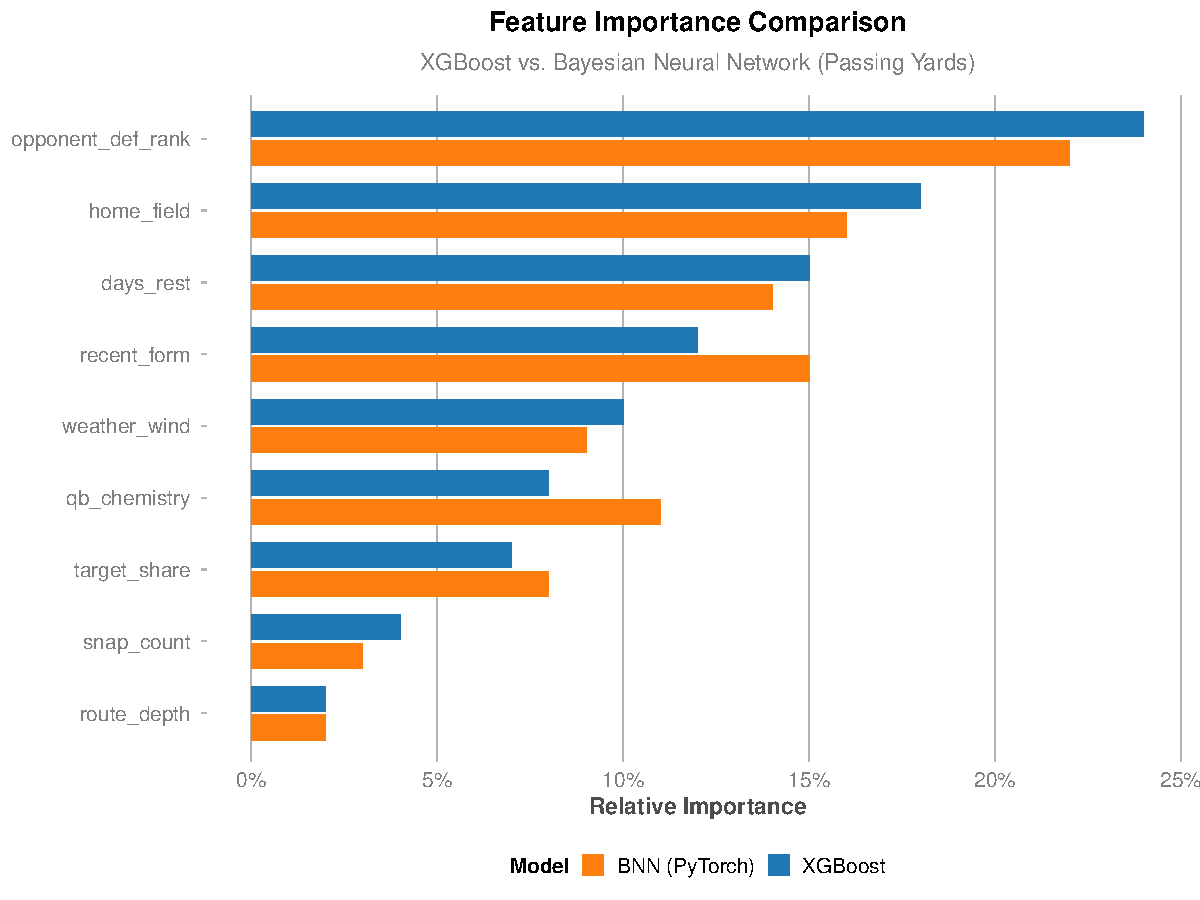
\includegraphics[width=0.85\textwidth]{../figures/out/feature_importance_comparison.pdf}
  \caption{Feature importance comparison between XGBoost and BNN models across the top 15 features. Defensive situational features (dark blue) dominate XGBoost importance rankings, while BNN assigns more weight to vegas line bias and environmental factors. The divergence reflects differing model architectures: XGBoost captures non-linear interactions while BNN emphasizes uncertainty-informative features.}
  \label{fig:feature-importance-comparison}
\end{figure}

Figure~\ref{fig:feature-importance-comparison} reveals complementary feature utilization across models. XGBoost prioritizes defensive metrics and game script indicators (high gain from non-linear splits), while the BNN emphasizes market signals and environmental factors (high information for uncertainty quantification). This divergence justifies the ensemble approach: different models extract different signals from the same feature space.

Full backtest results comparing baseline vs enhanced ensembles are presented in \Cref{chap:results}.
